% Provenance (never printed): see sources/outline_sources.md (Year 2: ancient massifs,
% Caledonian and Variscan belts; the Wilson cycle; supercontinents). Caledonian phases after
% McKerrow, Mac Niocaill and Dewey (2000) and Schiffer et al. (2020); the Wilson cycle after
% Chenin et al. (2018) and Schiffer et al. (2020); the Variscan belt after Faure (2024);
% supercontinents after Nance (2022); Siccar Point after the IUGS Geoheritage description.
% Model ocean and supercontinent chart from figdata/bachelor-2/wilson.py. Exercise and problem
% values in the Book 4 scratch calculator calc/ch15.py.
\chapter{الكتل القديمة ودورة ويلسون}\label{ch:b2:wilson-cycle}

على ساحل جنوب شرق اسكتلندا، عند سيكار بوينت، تقف طبقات رمادية من الحجر الرملي منتصبة
تحت غطاء من حجر رملي أحمر يميل ميلًا خفيفًا نحو البحر. ترسّبت الطبقات الرمادية في
محيط في بداية السيلوري، ثم طُويت واكتسبت انفصامًا حين انغلق ذلك المحيط؛ ثم حُتّت
حتى صارت سطحًا غير مستوٍ؛ وفي الديفوني المتأخر دفنتها حصى حمراء، وأمالت حركة
بناء جبلي ثانية، أهدأ، الطبقات الحمراء بدورها. فجرف واحد يسجّل محيطًا
زال، وحزامًا جبليًا اندثر، والحزام الذي تلاه. يقرأ هذا الفصل سجلات كهذه،
ويجمعها في دورة تتبعها الأحواض المحيطية، ثم يرجع خطوة إلى الوراء نحو أطول إيقاع على
الإطلاق، تجمّع القارات العظمى وتفكّكها.
% ledger: iugs:siccar-orogenies, iugs:siccar-point

\begin{recall}
\textbf{من مجلدات المدرسة}: بانجيا وتفكّكها، والقارات العظمى؛ وحالات عدم التوافق؛
ومعدّل التعرية، والارتداد الأيزوستاتي، والتناقص الأسّي لسلسلة جبلية تبريها
أنهارها. \textbf{من مجلد السنة الأولى}: الشقوق القارية، والهوامش السلبية
والظهرات وسط المحيطية، ومعدّلا التوسّع الكامل ونصفه؛ والاندساس والهوامش النشطة.
\textbf{من \cref{ch:b2:crustal-melting} إلى \cref{ch:b2:himalaya-andes}}: الميغماتيتات
والغرانيتات؛ \omterm{def:b2:alpine-orogen:orogen}{والأوروجين}، \omterm{def:b2:alpine-orogen:ophiolite}{والأوفيوليت}، والدرز، \omterm{def:b2:alpine-orogen:nappes}{والغطاء الزاحف}، \omterm{def:b2:alpine-orogen:foreland}{والفليش} \omterm{def:b2:alpine-orogen:foreland}{والمولاس}، \omterm{def:b2:alpine-orogen:foreland}{والحوض الأمامي الجبلي}؛ والأوروجينات التصادمية
والأنديزية النمط؛ \omterm{def:b2:himalaya-andes:thickening}{وتثخّن القشرة}، وسمك إيري \omterm{def:b2:himalaya-andes:collapse}{والانهيار الثقالي}.
\end{recall}

\begin{omfigure}
\centering
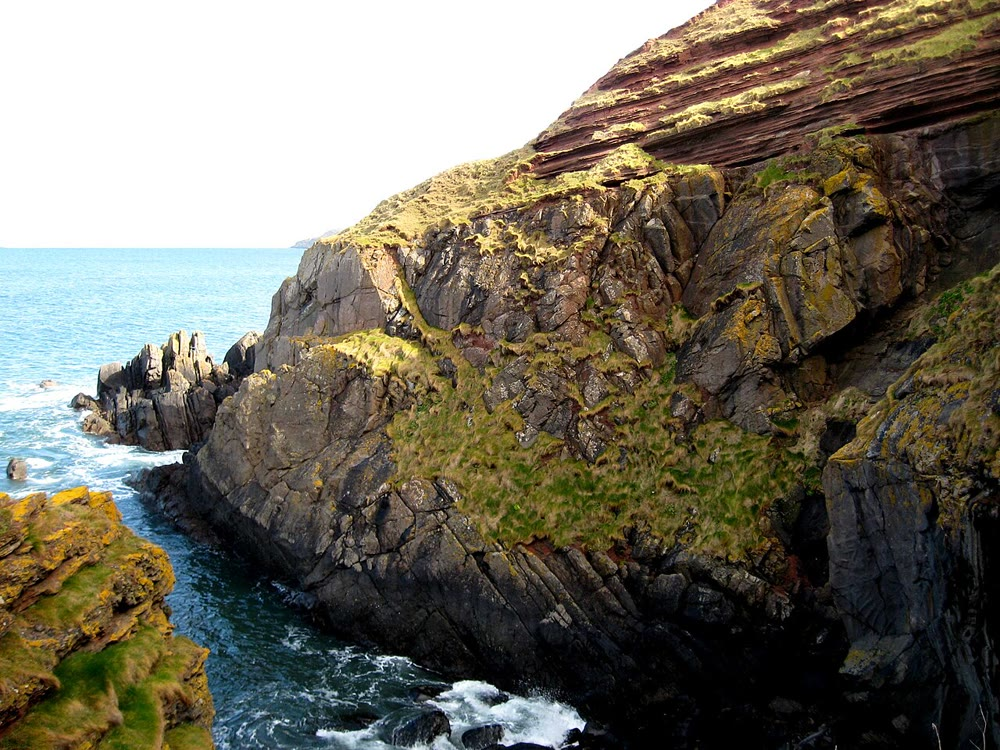
\includegraphics[width=0.64\linewidth]{images/book4/b2-15-siccar-point.jpg}
\par\smallskip{\small سيكار بوينت، من جنوب شرق الرأس: طبقات شبه رأسية من الغريواك الرمادي
السيلوري، طُويت في التكوّن الجبلي الكاليدوني، تحت طبقات حمراء خفيفة الميل من
الديفوني الأعلى. الصورة: \mbox{\textdir TLT dave souza, 2008, CC BY-SA 4.0}.}
\end{omfigure}
% ledger: iugs:siccar-orogenies

\section{أحزمة بُريت حتى جذورها}\label{sec:b2:wilson-cycle:old}

تعبر أوروبا الغربية وشرق أمريكا الشمالية أحزمة جبلية أقدم بكثير من
الألب. لقد زالت قممها، لكن صخورها باقية. ويهمّنا هنا ثلاثة منها.

يمتدّ الحزام \emph{الكاليدوني} من النرويج عبر اسكتلندا وأيرلندا إلى نيوفاوندلاند
وشمال الأبلاش، ويتواصل عبر شرق غرينلاند وسفالبارد. وهو سجلّ
محيط، إيابيتوس، كان يقع في أوائل الباليوزوي بين لورنتيا، سلف أمريكا
الشمالية وغرينلاند، في الشمال الغربي، وبلطيقا وأفالونيا في الجنوب الشرقي والشرق.
وكانت هوامشه قد انفصلت بالتصدّع الخسفي قبل نحو 600 مليون سنة؛ وأنتج انغلاقه، من الكامبري إلى
الديفوني، سلسلة كاملة من التصادمات، حتى إن التكوّن الجبلي الكاليدوني يمتدّ نحو
200 مليون سنة. فالمصطلح يسمّي مكانًا ومحيطًا، لا عصرًا.
% ledger: mckerrow00:caledonian, schiffer20:caledonides

والحزام \emph{الفاريسكي}، المسمّى الهرسيني في النصوص الأقدم، يعبر أوروبا من جنوب غرب
إنجلترا وبلجيكا عبر فرنسا وإيبيريا إلى وسط أوروبا؛ والحزام \emph{الأبلاشي} في
شرق أمريكا الشمالية توأمه الغربي. ويسجّلان معًا انغلاق المحيطات
بين القارة الجنوبية، غوندوانا، والقارة الشمالية، التي كانت قد التحمت للتوّ
بالتصادمات الكاليدونية. وقد خلّف آخر تصادماتهما، في الكربوني المتأخر والبرمي،
حزام طيّات يمتدّ شرقًا--غربًا عبر جنوب أوروبا وشمالًا شرقيًا--جنوبًا غربيًا بين
شرق أمريكا الشمالية وشمال غرب إفريقيا، ومعه \omterm{def:b2:wilson-cycle:supercontinent}{القارة العظمى} بانجيا.
% ledger: schiffer20:variscan, faure24:variscan

كيف يُتعرّف على حزام جبلي حُتّ ثلاثمئة مليون سنة؟
لا بتضاريسه، فقد زالت. بل يُبحث عن أجزائه، وكلٌّ منها التقته الفصول
السابقة:
\begin{itemize}
\item \emph{دروز} تحفّها \emph{الأوفيوليتات}، شرائح من قاع المحيط الذي انغلق؛
\item أحزمة من \emph{الصخور التحوّلية}، عالية الدرجة غالبًا، هي جذور القشرة المتثخّنة،
وقد صارت الآن على السطح لأن الكيلومترات التي كانت فوقها حُتّت؛
\item \emph{الغرانيتات} و\emph{الميغماتيتات}، نواتج الانصهار القشري الذي
يجلبه التثخّن والتسخين؛
\item رواسب المحيط المنغلق والحزام: \emph{\omterm{def:b2:alpine-orogen:foreland}{الفليش}} المُلقى في الأحواض العميقة
أثناء التقارب، و\emph{\omterm{def:b2:alpine-orogen:foreland}{المولاس}} المُلقى في الأحواض الأمامية والأحواض بين الجبلية؛
\item \emph{حالات عدم التوافق الزاوي}، حيث ترتكز طبقات أحدث على طبقات طُويت
وحُتّت قبلها، فتؤرّخ التشوّه الواقع بين الاثنتين.
\end{itemize}

\begin{definition}[شبه السهل]\label{def:b2:wilson-cycle:peneplain}
\emph{شبه السهل}\index{شبه السهل} سطح أرضي قليل التضاريس، قريب من مستوى قاعدة
الحتّ، مقطوع عبر صخور مختلفة الصلابة والبنية بحتّ طويل لتضاريس
سابقة.
\end{definition}

الحزام الفاريسكي أوروجين حارّ. ففي الألب في \cref{ch:b2:alpine-orogen}، اتّبعت الصخور
تدرّجات تحوّلية قدرها نحو \qty{8}{\celsius} لكل كيلومتر؛ أمّا في الحزام الفاريسكي،
فنحو \qty{30}{\celsius} لكل كيلومتر. وقد انصهرت قشرته على نطاق واسع: ففي الكتلة الوسطى الفرنسية
والكتلة الأرموريكية، تكوّنت الميغماتيتات بين نحو 330 و325 مليون سنة مضت،
واخترقتها الغرانيتات. وهذا الانصهار هو الفرق الرئيسي عن الألب الغربية. ومع
انتهاء التصادم، رقّت القشرة المتثخّنة بالتمدّد، وصعدت الصخور التحوّلية
على امتداد أسطح الانفصال، وانفتحت أحواض بين جبلية؛ ثم سوّى الحتّ السلسلة فصارت
\omterm{def:b2:wilson-cycle:peneplain}{شبه سهل} برمي وترياسي ترسّبت عليه رواسب الدورة التالية.
% ledger: faure24:variscan

\begin{omfigure}
\centering\small
\begin{tabular}{>{\raggedright\arraybackslash}p{0.2\linewidth}|>{\raggedright\arraybackslash}p{0.17\linewidth}|>{\raggedright\arraybackslash}p{0.52\linewidth}}
المرحلة & العمر & ما الذي تصادم \\ \hline
البنوبسكوتية & من 490 إلى \qty{485}{Ma} & قوس جزري دُسر على الهامش الأفالوني \\
الغرامبية، التاكونية & من 480 إلى \qty{455}{Ma} & أقواس جزرية في مواجهة لورنتيا (اسكتلندا؛ شمال الأبلاش) \\
الشلفية & أوائل الأوردوفيشي المتأخر & أفالونيا في مواجهة بلطيقا؛ بحر تورنكفيست ينغلق \\
الإسكاندية & من 425 إلى \qty{400}{Ma} & بلطيقا في مواجهة لورنتيا؛ الأغطية الزاحفة الكبرى في إسكندنافيا \\
الأكادية & الديفوني المبكر & \omterm{def:b2:wilson-cycle:terrane}{رقع قشرية} من غوندوانا في مواجهة القارة الجديدة؛ إيابيتوس انغلق \\
\end{tabular}
\par\smallskip{\small المراحل الرئيسية للتكوّن الجبلي الكاليدوني. المراحل المبكرة
تصادمات أقواس بأقواس أو بقارات، والمتأخرة تصادمات قارات؛ ومعظم
المراحل بدأت في أوقات مختلفة في أماكن مختلفة.}
\end{omfigure}
% ledger: mckerrow00:phases, schiffer20:caledonides

يُظهر الجدول الكاليدوني أعلاه السمة الأخرى للأحزمة القديمة: إنها مركّبة. فقبل أن
تلتقي القارتان، جاءت الأقواس والكتل الأصغر واحدة تلو الأخرى والتحمت بها.

\begin{definition}[الرقعة القشرية؛ القارة الصغرى]\label{def:b2:wilson-cycle:terrane}
\emph{الرقعة القشرية}\index{الرقعة القشرية} كتلة من القشرة تحدّها صدوع، يختلف تاريخها الجيولوجي
عن تاريخ جاراتها، وقد جاءت بها حركة الصفائح إلى موضعها الحالي؛ وقد
تكون قوسًا جزريًا، أو هضبة محيطية، أو شريحة من قاع المحيط، أو قطعة من قارة.
و\emph{القارة الصغرى}\index{القارة الصغرى} كتلة من القشرة القارية، أصغر من
قارة، تفصلها عن القارات قشرة محيطية.
\end{definition}

كانت أفالونيا كتلة من هذا النوع: شريط من القشرة غادر هامش غوندوانا، وفتح محيط
ريك خلفه في الأوردوفيشي، وعبر إيابيتوس ورسا على بلطيقا ثم على
لورنتيا. وتبعتها بدورهما أرموريكا وساكسوثورينجيا، الواقعتان اليوم في فرنسا وألمانيا؛ ودروزهما،
التي تحدّدها الأوفيوليتات، تقسم الحزام الفاريسكي إلى نطاقات من مقدّمة شمالية
في القارة الشمالية القديمة إلى مقدّمة جنوبية في غوندوانا.
% ledger: schiffer20:caledonides, schiffer20:variscan, faure24:variscan

\begin{omfigure}
\centering
\begin{tikzpicture}[x=0.5cm, y=0.5cm, font=\scriptsize]
\tikzset{cont/.style={fill=orange!25, draw=black!60, line width=0.4pt},
  terr/.style={fill=orange!45, draw=black!60, line width=0.4pt},
  ocn/.style={font=\scriptsize\itshape, text=blue!50!black},
  belt/.style={pattern=north east lines, pattern color=red!60!black, draw=red!60!black}}
% panel A
\begin{scope}
\fill[blue!6] (0,0) rectangle (9,8);
\draw[cont] (0.3,4.2) -- (3.0,4.0) -- (3.4,7.7) -- (0.3,7.7) -- cycle;
\node[align=center] at (1.7,6.0) {لورنتيا};
\draw[cont] (6.0,5.4) -- (8.7,5.0) -- (8.7,7.7) -- (6.4,7.7) -- cycle;
\node at (7.4,6.6) {بلطيقا};
\draw[cont] (0.3,0.3) -- (8.7,0.3) -- (8.7,1.6) -- (0.3,1.9) -- cycle;
\node at (4.5,0.95) {غوندوانا};
\draw[terr] (3.8,2.4) -- (6.6,2.2) -- (6.6,2.9) -- (3.8,3.1) -- cycle;
\node at (5.2,2.65) {أفالونيا};
\node[ocn] at (4.6,5.4) {إيابيتوس};
\node[ocn] at (7.7,2.55) {ريك};
\node[anchor=north west, font=\small\bfseries] at (0.1,8.9) {\foreignlanguage{arabic}{أ: نحو \qty{480}{Ma}}};
\end{scope}
% panel B
\begin{scope}[xshift=5.0cm]
\fill[blue!6] (0,0) rectangle (9,8);
\draw[cont] (0.3,3.6) -- (3.0,3.4) -- (3.4,7.7) -- (0.3,7.7) -- cycle;
\draw[cont] (3.0,3.4) -- (3.4,7.7) -- (8.7,7.7) -- (8.7,4.4) -- (5.2,4.6) -- (5.0,3.4) -- cycle;
\draw[terr] (3.0,3.4) -- (5.0,3.4) -- (5.2,4.6) -- (8.7,4.4) -- (8.7,3.6) -- (3.0,2.8) -- cycle;
\draw[red!60!black, line width=1.2pt] (3.0,3.4) -- (3.4,7.7);
\draw[red!60!black, line width=1.2pt] (5.0,3.4) -- (5.2,4.6) -- (8.7,4.4);
\node[align=center] at (1.6,5.6) {لورنتيا};
\node at (6.6,5.7) {بلطيقا};
\node at (6.4,3.75) {أفالونيا};
\node at (6.0,7.1) {\textbf{لوروسيا}};
\draw[cont] (0.3,0.3) -- (8.7,0.3) -- (8.7,1.3) -- (0.3,1.5) -- cycle;
\node at (4.5,0.8) {غوندوانا};
\draw[terr] (2.2,1.9) -- (3.6,1.9) -- (3.6,2.3) -- (2.2,2.3) -- cycle;
\draw[terr] (5.0,1.8) -- (6.6,1.8) -- (6.6,2.2) -- (5.0,2.2) -- cycle;
\node[ocn] at (7.7,2.3) {ريك};
\node[anchor=north west, font=\small\bfseries] at (0.1,8.9) {\foreignlanguage{arabic}{ب: نحو \qty{420}{Ma}}};
\end{scope}
% panel C
\begin{scope}[xshift=10.0cm]
\fill[blue!6] (0,0) rectangle (9,8);
\draw[cont] (0.3,3.0) -- (8.7,3.0) -- (8.7,7.7) -- (0.3,7.7) -- cycle;
\draw[cont] (0.3,0.3) -- (8.7,0.3) -- (8.7,3.0) -- (0.3,3.0) -- cycle;
\fill[belt] (0.3,2.5) -- (8.7,2.5) -- (8.7,3.5) -- (0.3,3.5) -- cycle;
\node[fill=orange!25, inner sep=1pt] at (4.5,5.6) {لوروسيا};
\node[fill=orange!25, inner sep=1pt] at (4.5,1.3) {غوندوانا};
\node[fill=white, fill opacity=0.85, text opacity=1, inner sep=1pt, align=center] at (4.5,3.0)
  {الحزام الفاريسكي--الأبلاشي};
\node[ocn] at (7.6,0.7) {};
\node[anchor=north west, font=\small\bfseries] at (0.1,8.9) {\foreignlanguage{arabic}{ج: نحو \qty{300}{Ma}، بانجيا}};
\end{scope}
\end{tikzpicture}
\par\smallskip{\small ثلاث لحظات من انغلاق محيطي إيابيتوس وريك، في صورة
رسم تخطيطي بلا إسقاط خرائطي ولا مقياس رسم: المواضع والأحجام والأشكال
طوبولوجية فقط. أ: غادرت أفالونيا غوندوانا وانفتح محيط ريك خلفها. ب: انغلق إيابيتوس؛
وتكوّن لورنتيا وبلطيقا وأفالونيا لوروسيا، على امتداد دروز كاليدونية (الخطوط الحمراء)؛
وكتل أصغر تعبر محيط ريك. ج: التقت غوندوانا بلوروسيا على امتداد
الحزام الفاريسكي--الأبلاشي (المخطّط).}
\end{omfigure}
% ledger: mckerrow00:caledonian, mckerrow00:phases, schiffer20:caledonides, schiffer20:variscan, faure24:variscan

\section{دورة ويلسون}\label{sec:b2:wilson-cycle:cycle}

في عام 1966 تساءل ج. توزو ويلسون عمّا إذا كان الأطلسي قد انغلق ثم
انفتح من جديد. فقد أخبرته أحافير الباليوزوي المبكر والأوسط أن محيطًا واسعًا كان يفصل حينها
حيوانات أمريكا الشمالية عن حيوانات أوروبا الغربية، وهو محيط لم يعد
موجودًا من أواخر الباليوزوي إلى أواسط الميزوزوي. وقد انفتح الأطلسي الحديث
قريبًا من الموضع الذي انغلق فيه ذلك المحيط الأقدم، إيابيتوس.
% ledger: schiffer20:wilson, chenin18:cycle

\begin{definition}[دورة ويلسون]\label{def:b2:wilson-cycle:wilson}
\emph{دورة ويلسون}\index{دورة ويلسون} تتابع المراحل التي ينفتح عبرها
حوض محيطي ثم ينغلق من جديد بين هوامش قارية: التصدّع الخسفي القاري،
فالانفصال وتوسّع قاع البحر، فمحيط يتّسع بهوامش سلبية، فبدء
الاندساس، فتضيّق المحيط وانغلاقه، فالتصادم القاري، فانهيار الحزام
وحتّه، وبعد ذلك قد تتصدّع القارة الملتحمة من جديد على امتداد النطاق نفسه.
\end{definition}

يتتبّع الشكل أدناه المراحل. وهي مراحل الفصول السابقة مرتّبة:
الشقوق والهوامش السلبية في مجلد السنة الأولى، والهوامش النشطة وأقواسها،
وتصادما الألب والهيمالايا، \omterm{def:b2:himalaya-andes:collapse}{والانهيار الثقالي} للتبت، والبري البطيء
للأحزمة القديمة.

\begin{omfigure}
\centering
\begin{tikzpicture}[x=0.38cm, y=0.38cm, font=\scriptsize]
\tikzset{crust/.style={fill=orange!25, draw=black!60, line width=0.3pt},
  ocrust/.style={fill=gray!45, draw=black!60, line width=0.3pt},
  sea/.style={fill=blue!8},
  ttl/.style={anchor=west, font=\scriptsize\bfseries}}
% 1 continent
\begin{scope}
\draw[crust] (0,0) -- (16,0) -- (16,2) -- (0,2) -- cycle;
\node[ttl] at (0,3.1) {\foreignlanguage{arabic}{1\enspace قارة}};
\end{scope}
% 2 rift
\begin{scope}[xshift=7.2cm]
\draw[crust] (0,0) -- (7,0) -- (7,2) -- (6.2,2) -- (5.4,1.0) -- (0,2) -- cycle;
\draw[crust] (9,0) -- (16,0) -- (16,2) -- (10.6,1.0) -- (9.8,2) -- (9,2) -- cycle;
\fill[red!50] (7,0) -- (9,0) -- (8.6,1.2) -- (7.4,1.2) -- cycle;
\draw[thick] (6.2,2) -- (7,0.4); \draw[thick] (9.8,2) -- (9,0.4);
\node[ttl] at (0,3.1) {\foreignlanguage{arabic}{2\enspace شقّ}};
\end{scope}
% 3 young ocean
\begin{scope}[yshift=-2.4cm]
\fill[sea] (5,2) -- (11,2) -- (11,0.6) -- (5,0.6) -- cycle;
\draw[crust] (0,0) -- (5,0) -- (6.2,0.5) -- (5,2) -- (0,2) -- cycle;
\draw[crust] (16,0) -- (11,0) -- (9.8,0.5) -- (11,2) -- (16,2) -- cycle;
\draw[ocrust] (6.2,0.5) -- (9.8,0.5) -- (9.8,0) -- (6.2,0) -- cycle;
\draw[red!70!black, thick] (8,0.5) -- (8,1.0);
\node[ttl] at (0,3.1) {\foreignlanguage{arabic}{3\enspace محيط فتيّ}};
\end{scope}
% 4 wide ocean
\begin{scope}[xshift=7.2cm, yshift=-2.4cm]
\fill[sea] (2.5,2) -- (13.5,2) -- (13.5,0.4) -- (2.5,0.4) -- cycle;
\draw[crust] (0,0) -- (2.5,0) -- (3.4,0.4) -- (2.5,2) -- (0,2) -- cycle;
\draw[crust] (16,0) -- (13.5,0) -- (12.6,0.4) -- (13.5,2) -- (16,2) -- cycle;
\draw[ocrust] (3.4,0.4) -- (12.6,0.4) -- (12.6,-0.4) -- (3.4,-0.4) -- cycle;
\draw[red!70!black, thick] (8,0.4) -- (8,0.9);
\node[anchor=north] at (3,-0.1) {سلبي};
\node[anchor=north] at (13,-0.1) {سلبي};
\node[ttl] at (0,3.1) {\foreignlanguage{arabic}{4\enspace محيط واسع}};
\end{scope}
% 5 subduction begins
\begin{scope}[yshift=-4.8cm]
\fill[sea] (2.5,2) -- (13.5,2) -- (13.5,0.4) -- (2.5,0.4) -- cycle;
\draw[crust] (0,0) -- (2.5,0) -- (3.4,0.4) -- (2.5,2) -- (0,2) -- cycle;
\draw[crust] (16,-0.4) -- (13.3,-0.4) -- (12.6,0.4) -- (13.5,2) -- (16,2) -- cycle;
\draw[ocrust] (3.4,0.4) -- (12.6,0.4) -- (11.6,-1.6) -- (3.4,-0.4) -- cycle;
\fill[red!60!black] (14.2,2) -- (14.6,2.7) -- (15.0,2) -- cycle;
\draw[red!70!black, thick] (7,0.4) -- (7,0.9);
\node[anchor=north] at (13.5,-0.5) {الخندق};
\node[ttl] at (0,3.1) {\foreignlanguage{arabic}{5\enspace بدء الاندساس}};
\end{scope}
% 6 ocean closes
\begin{scope}[xshift=7.2cm, yshift=-4.8cm]
\fill[sea] (5.5,2) -- (10.5,2) -- (10.5,0.4) -- (5.5,0.4) -- cycle;
\draw[crust] (0,0) -- (5.5,0) -- (6.4,0.4) -- (5.5,2) -- (0,2) -- cycle;
\draw[crust] (16,-0.4) -- (11.3,-0.4) -- (10.6,0.4) -- (11.5,2.4) -- (16,2.4) -- cycle;
\draw[ocrust] (6.4,0.4) -- (10.6,0.4) -- (9.4,-1.8) -- (6.4,-0.4) -- cycle;
\fill[red!60!black] (12.4,2.4) -- (12.8,3.1) -- (13.2,2.4) -- cycle;
\node[anchor=north west] at (11.6,-0.5) {قوس، خندق};
\node[ttl] at (0,3.1) {\foreignlanguage{arabic}{6\enspace المحيط ينغلق}};
\end{scope}
% 7 collision
\begin{scope}[yshift=-7.2cm]
\draw[crust] (0,0) -- (16,0) -- (16,2) -- (10,2) -- (8.6,3.6) -- (7.4,3.4) -- (6,2) -- (0,2) -- cycle;
\fill[crust] (5.6,0) -- (10.4,0) -- (9.6,-1.6) -- (6.4,-1.6) -- cycle;
\draw[black!60, line width=0.3pt] (5.6,0) -- (6.4,-1.6) -- (9.6,-1.6) -- (10.4,0);
\draw[red!60!black, line width=1pt] (8.6,3.6) -- (7.6,-1.6);
\node[anchor=west, text=red!60!black] at (9.0,3.5) {الدرز};
\node[ttl] at (0,3.1) {\foreignlanguage{arabic}{7\enspace التصادم}};
\end{scope}
% 8 worn flat
\begin{scope}[xshift=7.2cm, yshift=-7.2cm]
\draw[crust] (0,0) -- (16,0) -- (16,2) -- (0,2) -- cycle;
\draw[red!60!black, line width=1pt] (8.4,2) -- (7.6,0);
\fill[pink!60!red!40] (6.0,1.0) ellipse (0.7 and 0.4);
\node[anchor=north] at (8,-0.1) {شبه سهل فوق الجذر القديم};
\node[ttl] at (0,3.1) {\foreignlanguage{arabic}{8\enspace حزام مبريّ؛ قد يتبعه تصدّع خسفي}};
\end{scope}
\end{tikzpicture}
\par\smallskip{\small مراحل \omterm{def:b2:wilson-cycle:wilson}{دورة ويلسون}، في صورة مقاطع تخطيطية (دون مقياس رسم):
القشرة القارية بالبرتقالي، والقشرة المحيطية بالرمادي، والظهرة بالأحمر، وبراكين القوس في صورة
مثلثات؛ وفي اللوحة الأخيرة يبقى الدرز وغرانيت في قشرة ذات سمك عادي.}
\end{omfigure}
% ledger: chenin18:cycle, schiffer20:wilson

\subsection{ما العرض، وما المدّة؟}

ينمو المحيط بتوسّع قاع البحر عند ظهرته ويتقلّص بالاندساس عند خنادقه.
وحساب بسيط يعطي عرضه.

\begin{proposition}[عرض محيط عبر دورة]\label{prop:b2:wilson-cycle:width}
ليكن محيط ينفتح عند الزمن $t_0$ ويتّسع بمعدّل التوسّع الكامل $V_s$ لظهرته، حتى يبدأ
نطاق اندساس عند أحد الهامشين في الزمن $t_1$ ويستهلك قاع المحيط بالمعدّل $V_c$
بالنسبة إلى ذلك الهامش، مع $V_c > V_s$، والظهرة لا تزال تتوسّع. عرضه هو
\[
  W(t) = V_s\,(t - t_0) \quad (t_0 \le t \le t_1), \qquad
  W(t) = V_s\,(t_1 - t_0) - (V_c - V_s)\,(t - t_1) \quad (t \ge t_1),
\]
وهو أكبر ما يكون عند $t_1$، وينغلق المحيط بعد زمن قدره $V_s(t_1 - t_0)/(V_c - V_s)$ من بدء
الاندساس. ومع توسّع متناظر، تتحرّك الظهرة نحو الخندق بالسرعة $V_c - V_s/2$.
\end{proposition}

\begin{proof}
ثبّت الهامش الذي فيه الخندق. قبل $t_1$ يتباعد الهامشان بمعدّل
التوسّع الكامل $V_s$، فينمو العرض بالمعدّل $V_s$ من الصفر. وبعد $t_1$ تتحرّك الصفيحة الواقعة بين
الخندق والظهرة نحو الخندق بالسرعة $V_c$؛ وتضيف الظهرة $V_s$ إلى المسافة
بين تلك الصفيحة والصفيحة البعيدة، فيتحرّك الهامش البعيد نحو الخندق بالسرعة $V_c - V_s$،
وهو المعدّل الذي يتناقص به العرض. ويبلغ العرض الصفر بعد $V_s(t_1 - t_0)/(V_c -
V_s)$. ومع توسّع متناظر تتحرّك الظهرة بمتوسط سرعتي الصفيحتين على
جانبيها، $(V_c + (V_c - V_s))/2 = V_c - V_s/2$.
\end{proof}

يطبّق الشكل أدناه هذا الحساب على محيط نموذجي من نمط إيابيتوس: توسّع منذ
\qty{570}{Ma} بمعدّل \qty{30}{mm} في السنة، واندساس منذ \qty{490}{Ma} يستهلك \qty{60}{mm} في
السنة. والمعدّلات افتراضات، قيم مدوّرة من رتبة ما يُقاس اليوم في المحيطات؛
وإيابيتوس الحقيقي لم يكن بهذه البساطة ولا معروفًا إلى هذا الحدّ. ويبلغ المحيط النموذجي \qty{2400}{km}
وينغلق عند \qty{410}{Ma}، ضمن المدى الزمني للتصادم الإسكاندي.
% values (wilson.py): max_width_km 2400, closure_Ma 410; ledger: mckerrow00:caledonian, schiffer20:caledonides

\begin{omfigure}
\centering
% figdata/bachelor-2/wilson.py part ocean (model values: assumptions)
\begin{tikzpicture}
\begin{axis}[width=0.8\linewidth, height=5.0cm, x dir=reverse, xmin=360, xmax=600, ymin=0,
  ymax=3300, ytick={0,1000,2000,3000}, xlabel={العمر \babelsublr{(\unit{Ma})}}, ylabel={عرض المحيط \babelsublr{(\unit{km})}},
  tick label style={font=\scriptsize}, label style={font=\small}, xtick={600,560,...,360}]
\addplot[omThm, line width=1.2pt] table[x=t_Ma, y=width_km] {figdata/out/bachelor-2-wilson-ocean.dat};
\draw[dashed, black!50] (axis cs:490,0) -- (axis cs:490,2400);
\draw[dashed, black!50] (axis cs:570,0) -- (axis cs:570,2750);
\draw[dashed, black!50] (axis cs:410,0) -- (axis cs:410,2750);
\node[font=\scriptsize, anchor=south] at (axis cs:570,2750) {بدء التوسّع};
\node[font=\scriptsize, anchor=south west] at (axis cs:488,2400) {بدء الاندساس};
\node[font=\scriptsize, anchor=south] at (axis cs:410,2750) {التصادم};
\node[font=\scriptsize, anchor=west] at (axis cs:540,600) {\foreignlanguage{arabic}{انفتاح بالمعدّل $V_s$}};
\node[font=\scriptsize, anchor=south west, align=left] at (axis cs:446,1150) {\foreignlanguage{arabic}{انغلاق}\\\foreignlanguage{arabic}{بالمعدّل $V_c - V_s$}};
\end{axis}
\end{tikzpicture}
\par\smallskip{\small عرض محيط نموذجي عبر \omterm{def:b2:wilson-cycle:wilson}{دورة ويلسون} واحدة، من
\cref{prop:b2:wilson-cycle:width} مع $V_s = \qty{30}{mm}$ في السنة منذ \qty{570}{Ma} و$V_c
= \qty{60}{mm}$ في السنة منذ \qty{490}{Ma}. ويجري الزمن من اليسار إلى اليمين.}
\end{omfigure}

\subsection{الانفتاح حيث كان الانغلاق}

تستند فكرة ويلسون إلى فكرة ميكانيكية: الحزام القديم نطاق ضعف، والقارة التي
تُشدّ تميل إلى أن تنكسر على امتداد نطاقات ضعفها لا عبر داخلها القوي
المستقر.

\begin{definition}[إعادة التنشيط البنيوي]\label{def:b2:wilson-cycle:reactivation}
\emph{إعادة التنشيط البنيوي}\index{إعادة التنشيط البنيوي} لبنية سابقة
(صدع، أو نطاق قصّ، أو درز، أو تماس صخري) هي عودة تركّز
التشوّه على امتدادها، تحت حقل إجهاد لاحق قد يختلف عن الحقل الذي كوّنها.
\end{definition}

شمال الأطلسي هو حالة الاختبار، ولا ينجح فيه إلا جزئيًا. ففي وسط الأطلسي
يتبع المحيط الفتيّ جبال الأبلاش عن قرب. وبين إسكندنافيا وغرينلاند يتبع الانفصال
الحزام الكاليدوني إجمالًا. أمّا أبعد جنوبًا فلا: فدرز إيابيتوس لا يزال يمرّ
عبر شمال إنجلترا ووسط أيرلندا، وقد انفتح الأطلسي غربه، تاركًا
قطعًا من قشرة لورنتيا القديمة على الهامش الشمالي الغربي لأوروبا، حول روكول وهاتون.
وأبعد نحو الشمال الغربي، يقطع بحر لابرادور وخليج بافن مباشرة عبر كراتونات
وأحزمة أقدم. فالبنى القديمة توجّه الشقوق اللاحقة، لكن ليس دائمًا: فنطاق الضعف الذي برد أكثر
من 30 إلى 50 مليون سنة قد يكون صار قويًا، وقد يتبع شقّ جديد النسيج الأعمق
للوشاح بدلًا من الدرز القشري. \omterm{def:b2:wilson-cycle:wilson}{ودورة ويلسون} دليل، لا قانون.
% ledger: schiffer20:wilson, schiffer20:reactivation

ليست كل دورة تفتح محيطًا واسعًا. فكثير من الأوروجينات يغلق محيطات جنينية، شقوقًا لم
تكد تبدأ التوسّع، يقلّ عرضها عن نحو \qty{500}{km}: الألب، والبيرينيه، ومعظم
الحزام الفاريسكي في أوروبا الغربية. وأخرى تغلق محيطات واسعة ناضجة، كما فعلت
الكاليدونيات الإسكندنافية. ويظهر الفرق في النهاية. فالحزام الذي أغلق محيطًا واسعًا حمل
قوسًا طويل العمر، استنزف من الوشاح تحته جزءه القابل للانصهار؛ فكان انهياره فقيرًا
\omterm{def:b2:magma-emplacement:magma}{بالصهارة}، كما في الكاليدونيات. والحزام الذي أغلق حوضًا ضيقًا يقوم على وشاح خصب؛ فيمكن أن يكون
انهياره غنيًا \omterm{def:b2:magma-emplacement:magma}{بالصهارة}، كما في الحزام الفاريسكي، حيث الموهو اليوم مستوٍ
والقشرة السفلى طبقية، وهو ما يُقرأ بازلتًا مبطّنًا تحت القشرة أو قشرة سفلى قُصّت
وهي حارّة. وفي غضون بضع عشرات من ملايين السنين تخبو الشذوذات
الحرارية للحزام؛ وتبقى بناه.
% ledger: chenin18:cycle

\section{القارات العظمى}\label{sec:b2:wilson-cycle:supercontinents}

\begin{definition}[القارة العظمى؛ دورة القارات العظمى]\label{def:b2:wilson-cycle:supercontinent}
\emph{القارة العظمى}\index{القارة العظمى} كتلة يابسة تجمع معظم القشرة القارية
للأرض في كتلة واحدة. و\emph{دورة القارات العظمى}\index{دورة القارات العظمى} هي التجمّع
المتقطّع للقارات في قارة عظمى ثم تفكّكها
اللاحق، متكرّرًا عبر تاريخ الأرض.
\end{definition}

بانجيا، التي أعاد فيغنر بناءها ووصفتها مجلدات المدرسة، وُجدت من نحو 325
إلى 200 مليون سنة مضت. وقد اقتُرحت قارات عظمى أقدم: بانوتيا قبل نحو 620 إلى
580 مليون سنة، ووجودها موضع خلاف؛ ورودينيا قبل نحو 950 إلى 800 مليون سنة؛
ونونا، المسمّاة أيضًا كولومبيا، قبل نحو 1.6 إلى 1.4 مليار سنة؛ ثم، على نحو أقل يقينًا، كينورلاند
قبل نحو 2.7 إلى 2.5 مليار سنة وأُور قبل نحو 3.0 مليار سنة. ويبدو أنها
تجمّعت وتفكّكت بفواصل قدرها نحو نصف مليار سنة منذ ربما أواخر
الأركي. ورُبطت الدورة بأعمار البناء الجبلي، وبذُرى أعمار
الغرانيتات وحبيبات الزركون التي تحويها، وبنموّ القشرة، وبالمقاطعات النارية
الكبيرة، وبمستوى سطح البحر وبالمناخ: فتجمّع قارة عظمى يميل إلى أن يتزامن
مع التبرّد.
% ledger: nance22:supercontinents

\begin{omfigure}
\centering
% figdata/bachelor-2/wilson.py part supercontinents; ledger: nance22:supercontinents
\begin{tikzpicture}
\begin{axis}[width=0.86\linewidth, height=4.6cm, x dir=reverse, xmin=0, xmax=3300, ymin=-0.7,
  ymax=6.5, ytick=\empty, xlabel={العمر \babelsublr{(\unit{Ma})}}, tick label style={font=\scriptsize},
  label style={font=\small}, xtick={0,500,...,3000}, axis y line*=left,
  % labels: explicit nodes (the figdata table carries the English names)
  clip=false]
\addplot[only marks, mark=*, mark size=1.6pt, omThm,
  error bars/.cd, x dir=both, x explicit, error bar style={line width=3pt, omThm!60}, error mark=none]
  table[x=mid_Ma, y=row, x error=half_Ma] {figdata/out/bachelor-2-wilson-supercontinents.dat};
\node[font=\scriptsize, anchor=south, yshift=2pt] at (axis cs:3000,0) {أُور};
\node[font=\scriptsize, anchor=south, yshift=2pt] at (axis cs:2600,1) {كينورلاند};
\node[font=\scriptsize, anchor=south, yshift=2pt] at (axis cs:1500,2) {نونا--كولومبيا};
\node[font=\scriptsize, anchor=south, yshift=2pt] at (axis cs:875,3) {رودينيا};
\node[font=\scriptsize, anchor=south, yshift=2pt] at (axis cs:600,4) {بانوتيا};
\node[font=\scriptsize, anchor=south, yshift=2pt] at (axis cs:262.5,5) {بانجيا};
\end{axis}
\end{tikzpicture}
\par\smallskip{\small القارات العظمى عبر تاريخ الأرض، من التجمّع إلى التفكّك كما
أرّختها مراجعة حديثة: تمتدّ الأشرطة على الفترات المذكورة (لأُور تقدير واحد)،
والنقاط منتصفاتها. ووجود بانوتيا وكينورلاند وأُور موضع خلاف. ويجري الزمن من اليسار إلى اليمين.}
\end{omfigure}

هل الدورة دورية حقًا؟ إن منتصفات الفترات في المخطط تفصل بينها 400
و1100 و625 و275 و337.5 مليون سنة: أي نحو 550 في المتوسط، لكن بتشتّت قدره عامل
أربعة. فعبارة «نحو نصف مليار سنة» نزعة، لا ساعة، والقارات العظمى
الأقدم تستند إلى أدلّة شحيحة.
% values (wilson.py): spacings 400 1100 625 275 337.5, mean 547.5 Myr

\section{من الجبال إلى السهول}\label{sec:b2:wilson-cycle:erosion}

ما الذي يحوّل حزامًا كالهيمالايا إلى تلال بريتاني المنخفضة؟ لقد بنى مجلد المرحلة الثانوية
نموذجًا: تبري الأنهار السلسلة بمعدّل يتناسب مع متوسط ارتفاعها، $kh$،
وكل متر يُزال من القمة يُعاد جزء منه بالارتداد الأيزوستاتي، بحيث لا يُفقد ارتفاعًا
إلا الجزء $f = (\rho_m - \rho_c)/\rho_m$ منه. فيتناقص متوسط الارتفاع عندئذ
وفق
\[
  h(t) = h_0\,e^{-k f t} ,
\]
مع ثابت الزمن $\tau = 1/(kf)$. وفي الأحواض الكبيرة في العروض الوسطى، يتناسب معدّل التعرية
مع متوسط التضاريس، ودون رفع كانت التضاريس ستهبط إلى عُشر
قيمتها في نحو 11 مليون سنة: $k = \ln 10/11 \approx 0.21$ لكل مليون سنة. ومع
الكثافتين 2700 و\qty{3300}{kg.m^{-3}}، يكون $f = 0.18$ و$\tau \approx \qty{26}{Myr}$: فسلسلة
ارتفاعها \qty{3}{km} تظل مرتفعة \qty{1}{km} بعد نحو 30 مليون سنة، وتهبط
دون \qty{300}{m} بعد نحو 60 مليون سنة.
% ledger: ahnert70:decay; values (wilson.py): k 0.20933 /Myr, f 0.18182, tau 26.275 Myr

والارتداد نفسه يفسّر لماذا تكشف الأحزمة القديمة جذورها. فلإعادة قشرة متثخّنة من
$H$ إلى $T$ إلى مستوى سطح البحر، يجب حتّ السمك الإضافي كله $T - H$، بينما لم يكن متوسط
الارتفاع إلا $(T - H)f$: أي يُزال من الصخر نحو 5.5 أضعاف ارتفاع
السلسلة. فالصخور التي كانت على عمق 20 أو \qty{30}{km} في الجذر تصعد إلى السطح:
ميغماتيتات الكتل القديمة وغرانيتاتها ونيساتها عالية الدرجة، كتلك التي في الكتلة
الوسطى الفرنسية.
% ledger: ahnert70:decay

السلسلة الفاريسكية، التي انتهت آخر تصادماتها قبل نحو 290 مليون سنة، كانت قد
سُوّيت فصارت \omterm{def:b2:wilson-cycle:peneplain}{شبه سهل} خلال البرمي والترياسي: أي ضمن المدة التي يعطيها النموذج،
نحو 60 مليون سنة. ويمكن للانهيار أن يسرّع ذلك: فتمدّد قشرة متثخّنة، كما في
التبت اليوم، يرقّقها مباشرة، دون انتظار الأنهار. وعند سيكار بوينت، ترتكز حصى الديفوني المتأخر على
طبقات سيلورية طُويت في التصادمات الكاليدونية، فوق سطح أرضي قديم لا يزال يحتفظ
ببعض التضاريس بين الطبقات الصلبة والطبقات اللينة.
% ledger: faure24:variscan, iugs:siccar-orogenies

\begin{inthefield}[قراءة عدم توافق زاوي]
يبدأ الجيولوجيون الذين يدرسون عدم توافق زاويًا مثل سيكار بوينت بقياس
وضع الطبقات تحت السطح وفوقه، المضرب والميل، في أماكن كثيرة. ويبحثون
عن اتجاه أعلى الطبقات السفلى، بالتطبّق المتدرّج أو بالعلامات على قواعد الطبقات،
لأن الطبقات المطويّة قد تكون مقلوبة. ويفحصون السطح نفسه: تضاريسه،
والتجوية تحته، وحصى الصخور الأقدم في الكونغلوميرا فوقه. ثم يؤرّخون:
فأحدث الأحافير تحته تعطي العمر الذي لا يمكن أن يكون الطيّ قد حدث قبله،
وأقدم الأحافير فوقه العمر الذي كان الطيّ قد حدث قبله وكانت الأرض قد بُريت.
والفجوة بين الاثنين تحصر التكوّن الجبلي. وعند سيكار بوينت الطبقات السفلى من أوائل
السيلوري والعليا من الديفوني المتأخر، ويقع الطيّ والرفع والحتّ الكاليدونية
بينهما؛ أمّا الميل الخفيف للطبقات العليا فأحدث مرة أخرى، فاريسكي.
\end{inthefield}
% ledger: iugs:siccar-orogenies, ics:base.Silurian, ics:base.Devonian, ics:base.Carboniferous

\section*{التمارين}\label{sec:b2:wilson-cycle:exercises}

معطيات التمارين: $g = \qty{9.8}{m.s^{-2}}$؛ وكثافتا القشرة والوشاح
\qty{2700}{kg.m^{-3}} و\qty{3300}{kg.m^{-3}}؛ والقشرة العادية $H = \qty{35}{km}$؛ وأعمار
قواعد السيلوري والديفوني والكربوني 443.1 و419.6 و\qty{358.9}{Ma}، وقاعدة
الترياسي \qty{251.9}{Ma}.

\begin{exercise}[$\star$]\label{exo:b2:wilson-cycle:1}
انفصلت هوامش إيابيتوس قبل نحو \qty{600}{Ma}؛ وانتهى التصادم الكاليدوني الرئيسي،
الإسكاندي، قرب \qty{400}{Ma}؛ وبدأ أول تصادم بين قوس وقارة مع لورنتيا
قرب \qty{480}{Ma}. (أ) كم دامت دورة إيابيتوس كلها؟ (ب) كم دامت
التصادمات؟ (ج) لماذا لا ينبغي استعمال «كاليدوني» للدلالة على عمر؟
\end{exercise}

\begin{exercise}[$\star$]\label{exo:b2:wilson-cycle:2}
رتّب هذه الحالات وفق ترتيب \omterm{def:b2:wilson-cycle:wilson}{دورة ويلسون} وسمِّ مرحلة كلٍّ منها: (أ)
البحر الأحمر، محيط ضيق بين هامشين فتيّين متصدّعين؛ (ب) الهيمالايا؛ (ج) الشقّ
لشرق إفريقيا؛ (د) المحيط الأطلسي، الواسع، بهوامش سلبية على جانبيه؛ (ه) الهامش الهادئي
لأمريكا الجنوبية؛ (و) تلال بريتاني المنخفضة على قاعدة قديمة من الغرانيت والنيس.
\end{exercise}

\begin{exercise}[$\star$]\label{exo:b2:wilson-cycle:3}
عند سيكار بوينت تقع طبقات من أوائل السيلوري تحت طبقات من الديفوني المتأخر. (أ) بين أي حدّين،
تعطيهما المعطيات أعلاه، يجب أن يكون الطيّ والرفع والحتّ قد حدثت؟ (ب) ما
أطول زمن يمكن أن تكون قد استغرقته؟ (ج) عدّد بالترتيب الأحداث التي يسجّلها الجرف.
\end{exercise}

\begin{exercise}[$\star$]\label{exo:b2:wilson-cycle:4}
قل هل كلٌّ مما يلي \omterm{def:b2:wilson-cycle:terrane}{رقعة قشرية}، أم \omterm{def:b2:wilson-cycle:terrane}{قارة صغرى}، أم كلاهما، أم لا هذا ولا ذاك، ولماذا: (أ) أفالونيا؛
(ب) لورنتيا؛ (ج) قوس جزري التحم بقارة؛ (د) درز إيابيتوس.
\end{exercise}

\begin{exercise}[$\star\star$]\label{exo:b2:wilson-cycle:5}
خذ منتصفات فترات القارات العظمى أُور (3000)، وكينورلاند (2600)،
ونونا (1500)، ورودينيا (875)، وبانوتيا (600)، وبانجيا (262.5)، بملايين السنين قبل الحاضر.
(أ) احسب الفواصل الخمسة ومتوسطها. (ب) ما نسبة أكبر فاصل إلى
أصغرها؟ (ج) استبعد كينورلاند وأُور، وهما موضع شك: ما متوسط الفاصل بين
الأربع الأخرى؟ وهل «نصف مليار سنة» دور؟
\end{exercise}

\begin{exercise}[$\star\star$]\label{exo:b2:wilson-cycle:6}
يبدأ محيط عرضه \qty{3000}{km} بالاندساس عند أحد هامشيه بمعدّل \qty{70}{mm} في السنة،
بينما تتوسّع ظهرته بمعدّل \qty{25}{mm} في السنة. (أ) كم يستغرق انغلاقه؟
(ب) وكم يستغرق إذا توقّف التوسّع فورًا؟ (ج) حركة أي صفيحة تحدّد معدّل الانغلاق بعد
اندساس الظهرة؟
\end{exercise}

\begin{exercise}[$\star\star$]\label{exo:b2:wilson-cycle:7}
افترض أن الانصهار القشري يبدأ عند نحو \qty{700}{\celsius} وأن السطح عند
\qty{0}{\celsius}. (أ) على أي عمق تُبلغ تلك الحرارة على امتداد تدرّج قدره
\qty{8}{\celsius} لكل كيلومتر؟ وتدرّج قدره \qty{30}{\celsius} لكل كيلومتر؟ (ب) أي الحزامين، الألب
أم الحزام الفاريسكي، ينبغي عندئذ أن يكشف ميغماتيتات وغرانيتات قشرية المنشأ؟
(ج) لماذا يبالغ التدرّج الثابت في تقدير العمق في الحالة الأولى؟
\end{exercise}

\begin{exercise}[$\star\star$]\label{exo:b2:wilson-cycle:8}
انتهت التصادمات الفاريسكية قرب \qty{290}{Ma}؛ وكان \omterm{def:b2:wilson-cycle:peneplain}{شبه سهل} قد تكوّن بحلول البرمي
والترياسي. استعمل نموذج التناقص في الفصل، $\tau = \qty{26.3}{Myr}$. (أ) كم تستغرق
سلسلة لتهبط من متوسط ارتفاع قدره \qty{3}{km} إلى \qty{0.3}{km}؟ (ب) عند أي عمر يكون
ذلك؟ (ج) ما ثابت الزمن الذي يوصلها إلى هناك بحلول قاعدة الترياسي؟ (د) ما
العملية التي يمكن أن تقصّر الزمن؟
\end{exercise}

\begin{exercise}[$\star\star$]\label{exo:b2:wilson-cycle:9}
(أ) اشرح لماذا يُظهر درز إيابيتوس في شمال إنجلترا ووسط أيرلندا، والقشرة اللورنتية
قرب روكول، أن الأطلسي لم يُعد الانفتاح تمامًا على امتداد الدرز القديم.
(ب) ما الذي يتوقّع جيولوجي أن يجده في القاعدة القديمة على جانبي الدرز
في أيرلندا؟ (ج) بقيت الأبلاش تتشوّه حتى البرمي المبكر؛ وبدأ التصدّع الخسفي
بعد التكوّن الجبلي بنحو 80 مليون سنة. قارن بالمدة، من 30 إلى 50 مليون سنة، التي يصير بعدها
نطاق بارد أقوى من أن يُعاد تنشيطه.
\end{exercise}

\begin{exercise}[$\star\star\star$]\label{exo:b2:wilson-cycle:10}
محيط عرضه \qty{3000}{km} ظهرته في وسطه، على بعد \qty{1500}{km} من خندق
يستهلك الصفيحة الواقعة في جهته بمعدّل \qty{70}{mm} في السنة؛ والظهرة تتوسّع بمعدّل \qty{40}{mm} في
السنة، توسّعًا متناظرًا. (أ) بأي سرعة تقترب الظهرة من الخندق؟ (ب) متى
تبلغه؟ (ج) ما عرض المحيط حينئذ؟ (د) ماذا يحدث للقوس البركاني حين تندسّ
ظهرة؟
\end{exercise}

\begin{exercise}[$\star\star\star$]\label{exo:b2:wilson-cycle:11}
يُثخّن تصادم قشرة من \qty{35}{km} إلى \qty{60}{km}، معوَّضة على طريقة إيري.
(أ) ما متوسط الارتفاع، بحسب \cref{prop:b2:himalaya-andes:airy}؟ (ب) كم من الصخر يجب أن
يزيله الحتّ لإعادة السطح إلى مستوى سطح البحر بقشرة ذات سمك عادي؟
(ج) ما الضغط الصخري الذي كانت تتحمّله الصخور التي ينتهي بها المطاف على السطح؟ (د) في أي
سحنة تحوّلية يمكن أن تكون قد أعادت تبلورها؟
\end{exercise}

\begin{exercise}[$\star\star\star$]\label{exo:b2:wilson-cycle:12}
بعد التقاء قارتين، يستمر التقارب بمعدّل \qty{30}{mm} في السنة مدة \qty{10}{Myr}.
ويُستوعب التقصّر عبر حزام ينتهي عرضه إلى \qty{300}{km}، في قشرة كان
سمكها \qty{35}{km}. (أ) باستعمال \cref{prop:b2:himalaya-andes:shortening}، أوجد سمك
القشرة. (ب) أوجد ارتفاع إيري وجذره. (ج) باستعمال \cref{prop:b2:himalaya-andes:gpe}،
احسب فائض الطاقة الكامنة وقارنه بفائض التبت، \qty{6.1e12}{N.m^{-1}}.
(د) ما الذي ينبغي أن يلي ذلك؟
\end{exercise}

\begin{problem}[{مسألة نهاية الأسبوع --- إيابيتوس من الولادة إلى الموت}]\label{pb:b2:wilson-cycle:1}
ينفتح محيط نموذجي من نمط إيابيتوس بين قارتين، L في الشمال الغربي وB في
الجنوب الشرقي. يبدأ التصدّع الخسفي عند \qty{610}{Ma}؛ وتوسّع قاع البحر عند \qty{580}{Ma}.
وما لم يُذكر غير ذلك، $g = \qty{9.8}{m.s^{-2}}$ و$\rho_c = \qty{2700}{kg.m^{-3}}$ و$\rho_m =
\qty{3300}{kg.m^{-3}}$ وسمك القشرة العادية $H = \qty{35}{km}$. والتوسّع
متناظر ومعدّله ثابت.

\medskip
\noindent\textbf{الجزء الأول --- الانفتاح.}
\begin{enumerate}
\item عند \qty{500}{Ma}، يقع قاع محيط تكوّن عند \qty{540}{Ma} على بعد \qty{720}{km} من محور
الظهرة. احسب نصف معدّل التوسّع بالمليمترات في السنة.
\item استنتج معدّل التوسّع الكامل. إلى أي صنف من الظهرات ينتمي، بين الظهرات البطيئة
والسريعة وفائقة البطء؟
\item ما عرض المحيط عند \qty{540}{Ma}؟
\item وما عرضه عند \qty{500}{Ma}؟
\item ماذا افترض النموذج للحصول على هذين العرضين؟
\item ما عمر أقدم قاع محيطي عند \qty{500}{Ma}، وأين يقع؟ ولماذا هو
موضع مرجّح لبدء الاندساس؟
\end{enumerate}

\noindent\textbf{الجزء الثاني --- الانغلاق.} عند \qty{500}{Ma} يبدأ نطاق اندساس على امتداد
هامش L ويستهلك قاع المحيط بمعدّل \qty{64}{mm} في السنة بالنسبة إلى L؛ والظهرة تستمر في
التوسّع.
\begin{enumerate}[resume]
\item بأي معدّل يضيق المحيط؟
\item لو توسّعت الظهرة حتى النهاية، فمتى كان المحيط سينغلق؟
\item تبدأ الظهرة في وسط المحيط. متى تبلغ الخندق؟
\item ما عرض المحيط حينئذ؟
\item بعد أن تندسّ الظهرة، يتوقّف التوسّع وتقترب B من L بمعدّل \qty{40}{mm} في
السنة. متى ينغلق المحيط؟
\item قارن بأعمار المرحلة الإسكاندية، من 425 إلى \qty{400}{Ma}.
\end{enumerate}

\noindent\textbf{الجزء الثالث --- التصادم.} بعد التصادم، يستمر التقارب بمعدّل
\qty{40}{mm} في السنة مدة \qty{8}{Myr}؛ ويُستوعب التقصّر عبر حزام ينتهي عرضه إلى
\qty{400}{km}.
\begin{enumerate}[resume]
\item كم يبلغ هذا التقصّر؟
\item باستعمال \cref{prop:b2:himalaya-andes:shortening}، أوجد سمك القشرة.
\item باستعمال \cref{prop:b2:himalaya-andes:airy}، أوجد متوسط ارتفاعها وفق إيري وجذرها.
\item احسب فائض طاقتها الكامنة وقارنه بفائض التبت،
\qty{6.1e12}{N.m^{-1}}.
\item ماذا تتوقّع أن يفعل الحزام بعد ذلك؟
\end{enumerate}

\noindent\textbf{الجزء الرابع --- البري.} بحلول \qty{410}{Ma}، كان الانهيار قد خفض متوسط
الارتفاع إلى \qty{3.0}{km}. ثم يتبع الحتّ نموذج الفصل، مع $k = \ln
10/11$ لكل مليون سنة ومع الارتداد.
\begin{enumerate}[resume]
\item احسب $f$ وثابت الزمن $\tau$.
\item ما متوسط الارتفاع عند \qty{380}{Ma}؟
\item متى يهبط متوسط الارتفاع دون \qty{500}{m}؟
\item كم من القشرة الإضافية يُزال بينما يهبط من \qty{3.0}{km} إلى \qty{0.5}{km}؟
\item ما الضغط الصخري الذي تحمّلته في الجذر الصخورُ التي انكشفت حينئذ؟
\item ترتكز رواسب الديفوني المتأخر على الحزام المحتوت عند سيكار بوينت. هل توقيت النموذج
متّسق مع ذلك، علمًا بأن قاعدة الكربوني عند \qty{358.9}{Ma}؟
\item خلاصة: ما أكبر عرض بلغه المحيط النموذجي، بالكيلومترات؟
\end{enumerate}
\end{problem}
